\documentclass[11pt]{beamer}

\usepackage[english]{babel}
\usepackage{pgf}
\usepackage{amsmath,amssymb,wasysym}
\usepackage[latin1]{inputenc}
\usepackage{multirow}
\usepackage{graphicx}
\usepackage{ulem}
\usepackage{color}
\usepackage{hyperref}
% \usepackage{listings}

\mode<presentation>
{
  \useinnertheme{rectangles}
  \useoutertheme{split}
  \setbeamerfont{block title}{size={}}
  \usefonttheme{structurebold}
  \usecolortheme{Argonne}
  \setbeamercovered{transparent}
}

\pgfdeclareimage[width=3.0cm]{crest-logo}{ANL_V_White}
% \pgfdeclareimage[width=3.0cm]{crest-logo}{anl_logo2}
% \pgfdeclareimage[width=4.5cm]{crest-logo}{bgq-big}
% \pgfdeclareimage[width=4.5cm]{crest-logo}{images/merged-logos}
\titlegraphic{
    \pgfuseimage{crest-logo}
}

\title[NWChem Overview]{NWChem Overview}

\author[Jeff Hammond]{Jeff Hammond}

\institute[Argonne]{Leadership Computing Facility \\ Argonne National Laboratory}

\date[16 Nov 2011]{16 November 2011}

\definecolor{dgreen}{RGB}{0,150,0}
\definecolor{dred}{RGB}{200,0,0}

\begin{document}

\frame{\titlepage}

  \begin{frame}{NWChem 6.0 Overview} \Large
    \begin{itemize}
        \item \textbf{Open Source License:} \href{http://www.opensource.org/licenses/ecl2.php}{ECL 2.0} --- Apache 2.0 with patent modifications for academic users.
        \item \textbf{Wiki:} \href{http://www.nwchem-sw.org}{http://www.nwchem-sw.org}
        \item \textbf{Capability:} The most diverse collection of quantum chemical methodology of any code.  Notable missing features: TDDFT and CC analytic gradients.
        \item \textbf{Portability:} Runs on laptops/workstations (Linux, Mac and Cygwin), clusters (e.g. Fusion) and supercomputers (e.g. Intrepid and Jaguar).
    \end{itemize}
  \end{frame}

  \begin{frame}{Prerequisites} \Large
    Required:
    \begin{itemize}
        \item \textbf{Software:} \\ GNU/Linux environment or equivalent.
        \item \textbf{Hardware:} \\ A real computer (not a cell phone).
    \end{itemize}
    \vskip2ex
    If you want performance:
    \begin{itemize}
        \item \textbf{Software:} \\ MPI, BLAS, LAPACK, ScaLAPACK.
        \item \textbf{Hardware:} \\ Infiniband cluster or supercomputer.
    \end{itemize}
  \end{frame}

  \begin{frame}{Why Use NWChem?} \Large
    \begin{itemize}
        \item \textbf{Open Source:} Modify the code as needed.
        \item \textbf{Free:} Use anywhere.
        \item \textbf{Scalable:} No need to switch codes from laptop to supercomputer.
        \item \textbf{Functionality:} No need to use $N$ codes for 1 project.
        \item \textbf{Support:} Responsive developers and user community via \href{mailto:nwchem-users@emsl.pnl.gov}{nwchem-users@emsl.pnl.gov}.
        \item \textbf{Potential:} Actively developed by multiple DOE labs and user community.
    \end{itemize}
  \end{frame}

  \begin{frame}{} \LARGE
    \begin{center}
        \textbf{NWChem Highlight Reel}
    \end{center}
  \end{frame}

  \begin{frame}{Largest Coupled-cluster Excited-state Calculation} \Large
    \begin{figure}
        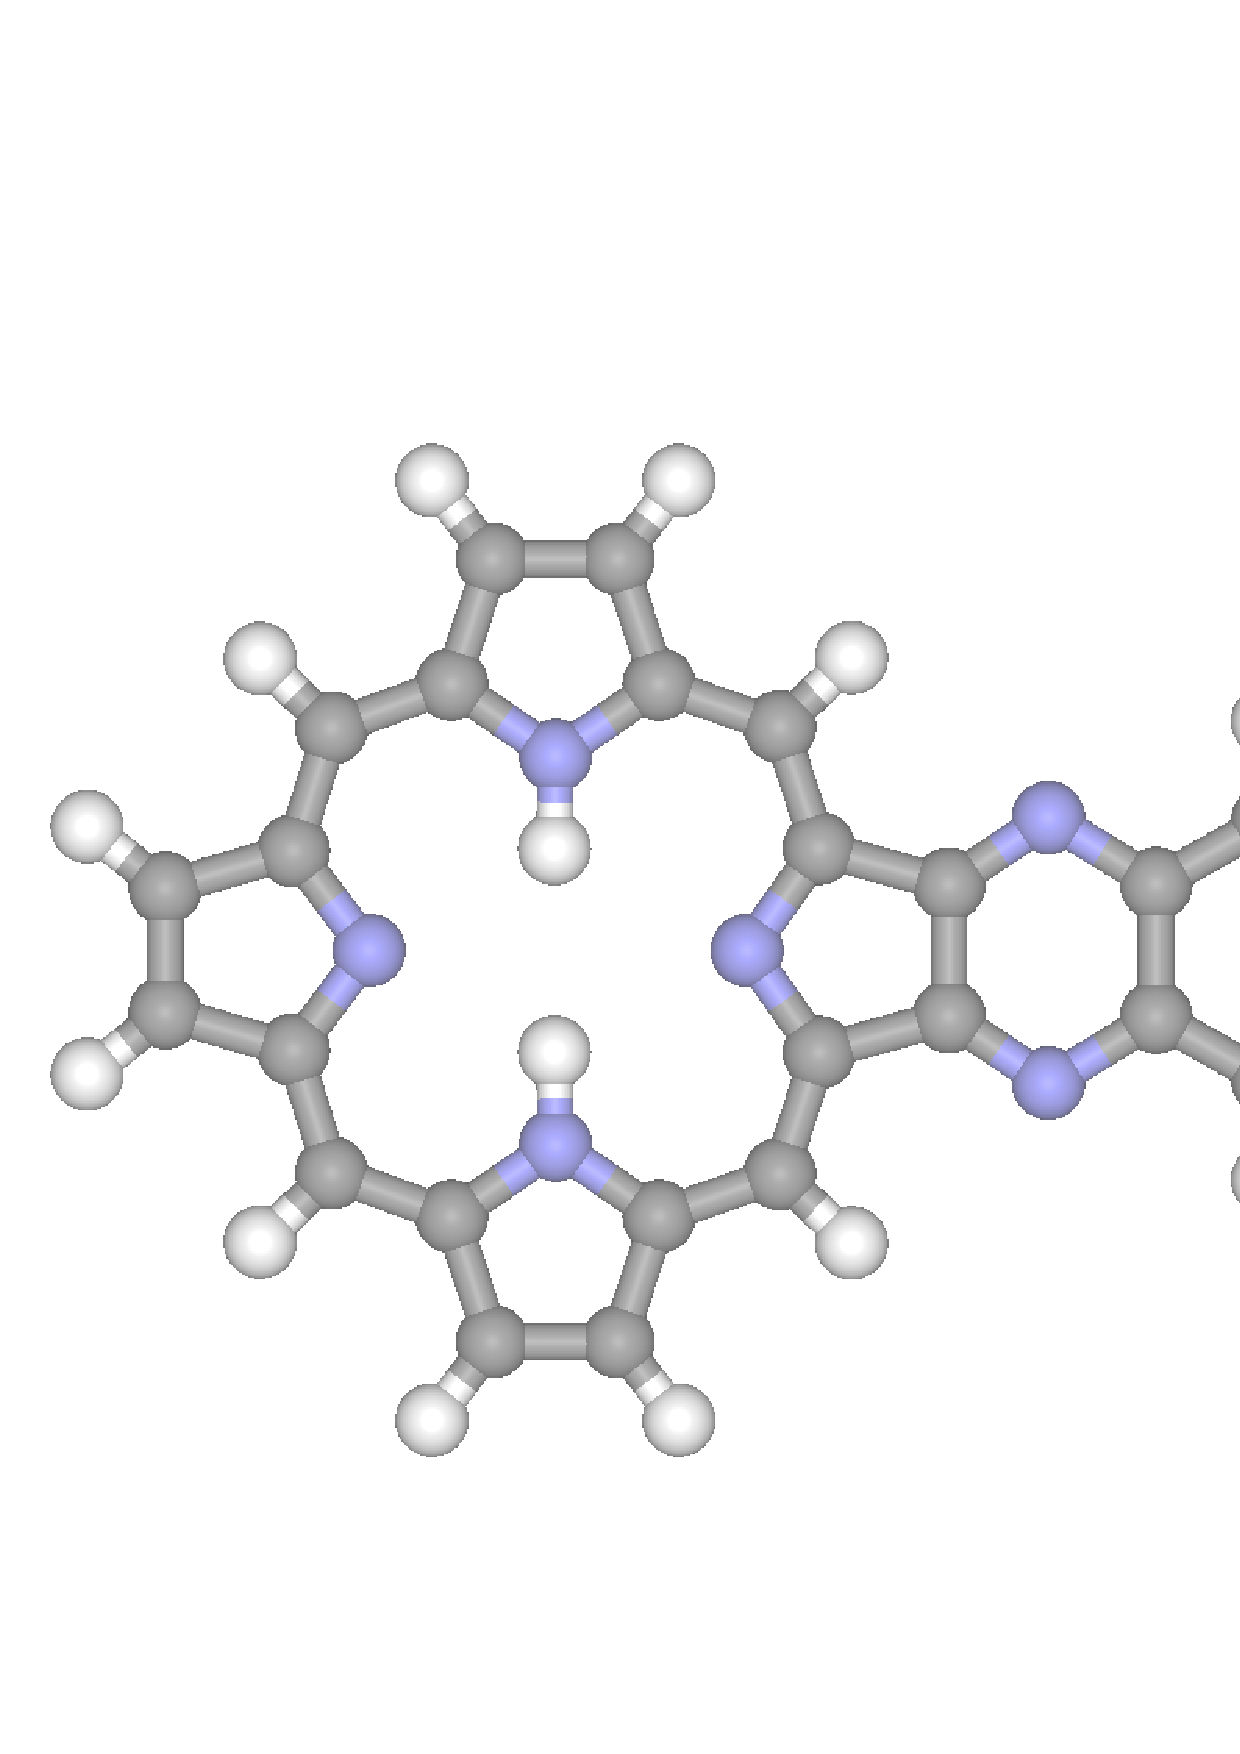
\includegraphics[scale=0.27,angle=0]{p2ta.png}
    \end{figure}
    \begin{center}\begin{tiny}
        \href{http://link.aip.org/link/JCPSA6/v132/i15/p154103/s1}{\textit{J. Chem. Phys.} \textbf{132}, 154103 (2010)}.
    \end{tiny}\end{center}
  \end{frame}

  \begin{frame}{Charge-transfer Excited-states of Biomolecules} \Large
    \begin{normalsize}
        CR-EOMCCSD(T)/6-31G* --- 1 hour on 256 cores
    \end{normalsize}
    \begin{figure}
        \includegraphics[scale=0.3,angle=0]{ANEPPS_scf_6-31pGs_orbitals-105-106.png}
    \end{figure}
    \begin{center}\begin{tiny}
        Joint work with Karol Kowalski (PNNL) and Beno\^{\i}t Roux (UC/Argonne).
    \end{tiny}\end{center}
  \end{frame}

  \begin{frame}{CCSD-LR Dynamic Polarizability} \Large
    \begin{normalsize}
        1080 b.f. --- 40 hours on 1024 processors
    \end{normalsize}
    \begin{figure}
    \includegraphics[scale=0.18,angle=90]{c60.jpg}
    \end{figure}
    \begin{center}\begin{tiny}
        \href{http://link.aip.org/link/jcpsa6/v129/i22/p226101/s1}{\textit{J. Chem. Phys.} \textbf{129}, 226101 (2008).}
    \end{tiny}\end{center}
  \end{frame}

  \begin{frame}{Large Fifth-rung DFT (B2PLYP)} \Large
    \begin{normalsize}
        2154 b.f. --- 7 hours on 256 cores
    \end{normalsize}
    \begin{figure}
        \vskip-1ex
        \includegraphics[scale=0.18]{stefan1.png}
    \end{figure}
    \begin{center}\begin{tiny}
        \textit{Organometallics} \textbf{29}, 1750-1760 2010.
    \end{tiny}\end{center}
  \end{frame}

  \begin{frame}{Large Hybrid DFT (PBE0)} \Large
    \begin{normalsize}
        no symmetry, 7560 b.f. --- 6 hours on 1024 cores
    \end{normalsize}
    \begin{figure}
        \includegraphics[scale=0.25]{c540_pbe0_6-31Gs.png}
    \end{figure}
  \end{frame}

  \begin{frame}{}\LARGE
    \begin{center}
      \textbf{Coupled-cluster theory}
    \end{center}
  \end{frame}

\begin{frame}{Coupled-cluster theory}
   The coupled--cluster (CC) wavefunction ansatz is
   \begin{equation}\nonumber
     \vert{CC}\rangle={e^T}\vert{HF}\rangle
   \end{equation}
   where $T=T_1+T_2+\cdots+T_n$. \\
   \vskip 1ex
   $T$ is an excitation operator which promotes $n$ electrons from occupied orbitals to virtual orbitals in the Hartree-Fock Slater determinant.
   \vskip 1ex
   Inserting $\vert{CC}\rangle$ into the Sch\"{o}dinger equation:
   \vskip-2ex
   \begin{columns}[T]
     \begin{column}{0.3\linewidth}
        \begin{equation}\nonumber
            \hat{H}{e^T}\vert{HF}\rangle = E_{CC}{e^T}\vert{HF}\rangle
        \end{equation}
     \end{column}
     \begin{column}{0.3\linewidth}
        \begin{equation}\nonumber
            \hat{H}\vert{CC}\rangle = E_{CC}\vert{CC}\rangle
        \end{equation}
     \end{column}
   \end{columns}
\end{frame}

  \begin{frame}{Coupled-cluster theory}
     \begin{eqnarray}
       \vert{CC}\rangle &=& \exp(T)\vert{0}\rangle \nonumber \\
       T &=& T_1+T_2+\cdots+T_n~~(n \ll N) \nonumber \\
       T_1 &=& \sum_{ia} t_i^a \hat{a}^{\dagger}_a \hat{a}_i \nonumber \\
       T_2 &=& \sum_{ijab} t_{ij}^{ab} \hat{a}^{\dagger}_{a} \hat{a}^{\dagger}_{b} \hat{a}_{j} \hat{a}_{i} \nonumber \\
       \vert{\Psi_{CCD}}\rangle  &=& \exp(T_2)\vert{\Psi_{HF}}\rangle \nonumber \\
                                 &=&(1+T_2+T_2^2)\vert{\Psi_{HF}}\rangle \nonumber \\
       \vert{\Psi_{CCSD}}\rangle &=& \exp(T_1+T_2)\vert{\Psi_{HF}}\rangle \nonumber \\
                                 &=&(1+T_1+\cdots+T_1^4+T_2+T_2^2+T_1 T_2+T_1^2 T_2)\vert{\Psi_{HF}}\rangle \nonumber \\
       \nonumber
     \end{eqnarray}
  \end{frame}

\begin{frame}{Coupled-cluster theory}
   Projective solution of CC: \vskip-3ex
   \begin{eqnarray}
     E_{CC} &=& \langle{HF}\vert{e^{-T}}{H}{e^T}\vert{HF}\rangle \nonumber \\
     0      &=&  \langle{X}\vert{e^{-T}}{H}{e^T}\vert{HF}\rangle~~~(X=S,D,\ldots) \nonumber
   \end{eqnarray}
    CCD is: \vskip-5ex
   \begin{eqnarray}
     E_{CC} &=& \langle{HF}\vert{e^{-T_2}}{H}{e^{T_2}}\vert{HF}\rangle \nonumber \\
     0      &=&  \langle{D}\vert{e^{-T_2}}{H}{e^{T_2}}\vert{HF}\rangle \nonumber
   \end{eqnarray}
    CCSD is: \vskip-5ex
   \begin{eqnarray}
     E_{CC} &=& \langle{HF}\vert{e^{-T_1-T_2}}{H}{e^{T_1+T_2}}\vert{HF}\rangle \nonumber \\
     0      &=&  \langle{S}\vert{e^{-T_1-T_2}}{H}{e^{T_1+T_2}}\vert{HF}\rangle \nonumber \\
     0      &=&  \langle{D}\vert{e^{-T_1-T_2}}{H}{e^{T_1+T_2}}\vert{HF}\rangle \nonumber
   \end{eqnarray}
\end{frame}

\begin{frame}{Notation}
   \begin{eqnarray}
     H &=& H_1 + H_2 \nonumber \\
       &=& F + V \nonumber
   \end{eqnarray}
    $F$ is the Fock matrix.  CC only uses the diagonal in the canonical formulation.
    \vskip1ex
    $V$ is the fluctuation operator and is composed of two-electron integrals as a 4D array.
    \vskip1ex
    $V$ has 8-fold permutation symmetry in $V_{pq}^{rs}$ and is divided into six blocks:
    $V_{ij}^{kl}$, $V_{ij}^{ka}$, $V_{ia}^{jb}$, $V_{ij}^{ab}$, $V_{ia}^{bc}$, $V_{ab}^{cd}$.
    \vskip1ex
    Indices $i,j,k,\ldots$ ($a,b,c,\ldots$) run over the occupied (virtual) orbitals.
\end{frame}

\begin{frame}{CCD Equations}
    \begin{eqnarray}\nonumber
        R_{ij}^{ab} =  V_{ij}^{ab} + P(ia,jb) \bigg[ T_{ij}^{ae} I_e^b - T_{im}^{ab} I_j^m + \frac{1}{2} V_{ef}^{ab} T_{ij}^{ef} + \nonumber \\
        \frac{1}{2} T_{mn}^{ab} I_{ij}^{mn} - T_{mj}^{ae} I_{ie}^{mb} - I_{ie}^{ma} T_{mj}^{eb} + (2 T_{mi}^{ea} - T_{im}^{ea}) I_{ej}^{mb} \bigg] \nonumber
    \end{eqnarray}
    \begin{eqnarray}
        I_b^a &=& (-2 V_{eb}^{mn} + V_{be}^{mn}) T_{mn}^{ea} \nonumber \\
        I_j^i &=& (2 V_{ef}^{mi} - V_{ef}^{im}) T_{mj}^{ef} \nonumber \\
        I_{kl}^{ij} &=& V_{kl}^{ij} + V_{ef}^{ij} T_{kl}^{ef} \nonumber \\
        I_{jb}^{ia} &=& V_{jb}^{ia} - \frac{1}{2} V_{eb}^{im} T_{jm}^{ea} \nonumber \\
        I_{bj}^{ia} &=& V_{bj}^{ia} + V_{be}^{im} (T_{mj}^{ea} - \frac{1}{2} T_{mj}^{ae}) - \frac{1}{2} V_{be}^{mi} T_{mj}^{ae} \nonumber
    \end{eqnarray}
\end{frame}

\begin{frame}{Turning CC into MMM}
 \begin{columns}[T]
  \begin{column}{0.45\linewidth}
    Some tensor contractions are trivially mapped to GEMM:
    \begin{eqnarray}
        I_{kl}^{ij} &+=& V_{ef}^{ij} T_{kl}^{ef} \nonumber \\
        I_{(kl)}^{(ij)} &+=& V_{(ef)}^{(ij)} T_{(kl)}^{(ef)} \nonumber \\
        I_{a}^{b} &+=& V_{c}^{b} T_{a}^{c} \nonumber
    \end{eqnarray}
   \end{column}
   \begin{column}{0.45\linewidth}
    Other contractions require reordering to use BLAS:
    \begin{eqnarray}
        I_{bj}^{ia} &+=& V_{be}^{im} T_{mj}^{ea} \nonumber \\
        I_{bj,ia} &+=& V_{be,im} T_{mj,ea} \nonumber \\
        J_{bi,ja} &+=& W_{bi,me} U_{me,ja} \nonumber \\
        J_{bi}^{ja} &+=& W_{bi}^{me} U_{me}^{ja} \nonumber \\
        J_{(bi)}^{(ja)} &+=& W_{(bi)}^{(me)} U_{(me)}^{(ja)} \nonumber \\
        J_{x}^{z} &+=& W_{x}^{y} U_{y}^{z} \nonumber
    \end{eqnarray}
   \end{column}
  \end{columns}
\end{frame}



%
%   \begin{frame}{} \LARGE
%     \begin{center}
%         \textbf{Creating NWChem Input Files}
%     \end{center}
%   \end{frame}
%
%   \begin{frame}{Input File Structure} \large
%     \begin{columns}[t]
%         \begin{column}{0.50 \linewidth}
%             \begin{tt}\\
%                 echo \\
%                 \vskip1ex
%                 start water \\
%                 \vskip1ex
%                 geometry \\
%                 ~~O  ~0.00  ~0.00  ~0.12 \\
%                 ~~H  ~0.75  ~0.00  -0.47 \\
%                 ~~H  -0.75  ~0.00  -0.47 \\
%                 end \\
%                 \vskip1ex
%                 basis \\
%                 ~~* library 6-31G \\
%                 end \\
%                 \vskip1ex
%                 task scf optimize \\
%             \end{tt}
%         \end{column}
%         \begin{column}{0.50 \linewidth}
%             \begin{block}{\texttt{echo}}<2->
%                 \color{dred}{Copies input into output.}
%             \end{block}
%             \begin{block}{\texttt{start <prefix>}}<3->
%                 \color{dred}{Names job, creates/overwrites existing files.}
%             \end{block}
%             \begin{block}{\texttt{geometry} and \texttt{basis}}<4->
%                 \color{dred}{Basic input blocks.}
%             \end{block}
%             \begin{block}{\texttt{task <method> <task>}}<5->
%                 \color{dred}{Initiates a calculation.}
%             \end{block}
%         \end{column}
%     \end{columns}
%   \end{frame}
%
%   \begin{frame}{} \LARGE
%     \begin{center}
%         \textbf{Geometry Input}
%     \end{center}
%   \end{frame}
%
%   \begin{frame}{Geometry Input --- Cartesian} \Large
%     \begin{tt}
%         geometry units angstroms autosym \\
%         ~~O  ~0.00  ~0.00  ~0.12 \\
%         ~~H  ~0.75  ~0.00  -0.47 \\
%         ~~H  -0.75  ~0.00  -0.47 \\
%         end \\
%     \end{tt}
%     \vskip2ex
%     \begin{block}{Other keywords of interest}<2->
%         \texttt{noautosym}, \texttt{units <bohr, pm, nm, atomic>}
%     \end{block}
%   \end{frame}
%
%   \begin{frame}{Geometry Input --- Simple Z-Matrix} \Large
%     \begin{tt}
%         geometry units angstrom  \\
%         ~symmetry c1 \\
%         ~zmatrix \\
%         ~~O \\
%         ~~H1 O 0.9572 \\
%         ~~H2 O 0.9572 H1 104.52 \\
%         ~end \\
%         end \\
%     \end{tt}
%   \end{frame}
%
%   \begin{frame}{Geometry Input --- Detailed Z-Matrix} \Large
%     \vskip1ex
%     \begin{tt}
%         geometry units angstrom autosym \\
%         ~zmatrix \\
%         ~~O \\
%         ~~H1 O r \\
%         ~~H2 O r H1 theta \\
%         ~~constants \\
%         ~~~theta 104.0 \\
%         ~~variables \\
%         ~~~r 0.95 \\
%         ~end \\
%         end \\
%     \end{tt}
%   \end{frame}
%
%   \begin{frame}{Geometry Input --- Constrained Internal Coordinates} \Large
%     \begin{tt}
%         geometry units angstroms autosym \\
%         ~~O  ~0.00  ~0.00  ~0.12 \\
%         ~~H  ~0.75  ~0.00  -0.47 \\
%         ~~H  -0.75  ~0.00  -0.47 \\
%         ~~zcoord \\
%         ~~~~angle 2 1 3 90.0 theta constant \\
%         ~~end \\
%         end \\
%     \end{tt}
%   \end{frame}
%
%   \begin{frame}{Geometry Input --- Forcing Symmetry} \Large
%     TCE only handles subgroups of $D_{2h}$, hence you need to forcibly reduce symmetry:
%     \vskip1ex
%     \begin{tt}
%         geometry units angstroms autosym \\
%         ~~symmetry d2h \\
%         ~~Ne 0.0 0.0 0.0 \\
%         end \\
%     \end{tt}
%     \vskip2ex
%     On the other hand, using symmetry ``fill in'' helps to construct e.g. $C_{60}$.
%   \end{frame}
%
%   \begin{frame}{Geometry Input --- Other Considerations} \Large
%     Consult the documentation regarding:
%     \begin{itemize}
%         \item symmetry group keywords
%         \item adding point charges
%         \item periodic geometries
%         \item changing mass, charge and extent of nuclei
%         \item naming geometries (useful for e.g. BSSE)
%         \item other obscure options
%     \end{itemize}
%   \end{frame}
%
%   \begin{frame}{} \LARGE
%     \begin{center}
%         \textbf{Basis Set Input}
%     \end{center}
%   \end{frame}
%
%   \begin{frame}{Basis Set Input --- Using the Library} \Large
%     \begin{columns}[t]
%         \begin{column}{0.45 \linewidth}
%             \begin{tt}\\
%                 basis cartesian\\
%                 ~* library 6-31G \\
%                 end \\
%             \end{tt}
%             \vskip1ex
%             \begin{tt}
%                 basis spherical \\
%                 ~C library cc-pVQZ \\
%                 ~H library cc-pVTZ \\
%                 end \\
%             \end{tt}
%         \end{column}
%         \begin{column}{0.55 \linewidth}
%             \begin{block}{\texttt{spherical} or \texttt{cartesian}}<2->
%                 \color{dred}{Pople $\rightarrow$ \texttt{cartesian}. \\ Dunning $\rightarrow$ \texttt{spherical}.}
%             \end{block}
%             \begin{block}{\texttt{library}}<3->
%                 \color{dred}{Specify all or by element.}
%             \end{block}
%         \end{column}
%     \end{columns}
%     \vskip3ex
%     NWChem library is extensive but missing some basis sets present in Gaussian.
%   \end{frame}
%
%   \begin{frame}{Basis Set Input --- Explicit Definition} \Large
%     \begin{tt}
%         basis \\
%         ~~H    S \\
%         ~~~33.8650140  0.0060680 \\
%         ~~~~5.0947880  0.0453160 \\
%         ~~H    S \\
%         ~~~~0.1027410  1.0000000 \\
%         ~~H    P \\
%         ~~~~1.1588000  0.1884400 \\
%         ~~~~0.3258000  0.8824200 \\
%         end \\
%     \end{tt}
%     \vskip1ex
%     Cut-and-paste from \href{https://bse.pnl.gov/bse/portal}{bse.pnl.gov/bse/portal}!
%   \end{frame}
%
%   \begin{frame}{Basis Set Input --- RI-MP2 Fitting Basis Sets} \Large
%     \begin{tt}
%         basis "ao basis" spherical \\
%         ~* library aug-cc-pVTZ \\
%         end \\
%         \vskip1ex
%         basis "ri-mp2 basis" spherical \\
%         ~* library cc-pVTZ-RI \\
%         ~* library aug-cc-pVTZ-RI\_diffuse \\
%         end \\
%     \end{tt}
%     \vskip2ex
%     This is how you activate RI-MP2 in NWChem.
%   \end{frame}
%
%   \begin{frame}{Basis Set Input --- DFT Fitting Basis Sets} \Large
%     \begin{tt}
%         basis "ao basis" cartesian \\
%         ~* library 6-31+G* \\
%         end \\
%         \vskip1ex
%         basis "cd basis" spherical \\
%         ~* library "Ahlrichs Coulomb Fitting" \\
%         end \\
%     \end{tt}
%     \vskip2ex
%     \begin{block}{When to Use Density-Fitting}<2->
%         Useful for GGA functionals (e.g. PBE). \\
%         Less useful for hybrid DFT (e.g. B3LYP).
%     \end{block}
%   \end{frame}
%
%   \begin{frame}{Basis Set Input --- Using ECPs} \Large
%     \begin{tt}
%         basis \\
%         ~Ca      library "lanl2dz ecp" \\
%         ~F       library "6-31g" \\
%         ~H       library "sto-3g" \\
%         end \\
%         \vskip1ex
%         ecp \\
%         ~Ca      library "lanl2dz ecp" \\
%         end \\
%     \end{tt}
%   \end{frame}
%
%   \begin{frame}{} \LARGE
%     \begin{center}
%         \textbf{Task Input}
%     \end{center}
%   \end{frame}
%
%   \begin{frame}{Task Input --- What is Available?} \Large
%     \begin{itemize}
%         \item energy
%         \item gradient/optimize/saddle/dynamics
%         \item hessian/frequencies
%         \item property
%         \item dplot
%         \item \textit{python}
%         \item \textit{shell}
%     \end{itemize}
%   \end{frame}
%
%   \begin{frame}{} \LARGE
%     \begin{center}
%         \textbf{Method Input}
%     \end{center}
%   \end{frame}
%
%   \begin{frame}{Method Input --- What is Available?} \Large
%     \begin{itemize}
%         \item SCF/DFT energy, gradient, hessian, property
%         \item TDDFT excited-state energy
%         \item MP2 energy and gradient (semidirect algorithm)
%         \item DHDF and RI-MP2 energy
%         \item CCSD/CCSD(T) energy (direct algorithm)
%         \item TCE energy (+properties), gradient (sort-of)
%         \item MCSCF energy, gradient and property
%     \end{itemize}
%   \end{frame}
%
%   \begin{frame}{} \LARGE
%     \begin{center}
%         \textbf{SCF Input}
%     \end{center}
%   \end{frame}
%
%   \begin{frame}{SCF Input --- Disk Usage} \Large
%     \begin{tt}
%         scf \\
%         ~~semidirect memsize <words> filesize 0\\
%         end \\
%     \end{tt}
%     \begin{columns}[t]
%         \begin{column}{0.3 \linewidth}
%             \vskip0ex
%             \begin{tt}
%                 scf \\
%                 ~~direct \\
%                 end \\
%             \end{tt}
%         \end{column}
%         \begin{column}{0.6 \linewidth}
%             \begin{block}{\texttt{semidirect}}<2->
%                 \color{black}{Use memory but not disk.}
%             \end{block}
%             \begin{block}{\texttt{direct}}<3->
%                 \color{black}{Compute integrals on-the-fly.}
%             \end{block}
%         \end{column}
%     \end{columns}
%     \vskip3ex
%     \vskip1ex
%     A word is 8 bytes.  Divide stack (in bytes) by 10.
%   \end{frame}
%
%   \begin{frame}{SCF Input --- Basic MOVEC I/O} \large
%     This is the default behavior: \\
%     \begin{tt}
%         scf \\
%         ~~vectors input atomic output <prefix>.movecs \\
%         end \\
%     \end{tt}
%     \vskip2ex
%     Read input guess: \\
%     \begin{tt}
%         scf \\
%         ~~vectors input <file> \\
%         end \\
%     \end{tt}
%     \vskip2ex
%     For geometry optimizations and restart, the second option is automatic.
%     \vskip1ex
%     You can use SCF, DFT and MCSCF movecs interchangeably.
%   \end{frame}
%
%   \begin{frame}{SCF Input --- Advanced MOVEC I/O} \large
%     \begin{tt}
%         basis "small" ; * library 3-21G ; end \\
%         basis "large" ; * library cc-pVTZ ; end \\
%         \vskip1ex
%         set "ao basis" "small" \\
%         scf \\
%         ~~vectors output <file> \\
%         end \\
%         task scf \\
%         \vskip1ex
%         set "ao basis" "large" \\
%         scf \\
%         ~~vectors input project "small" <file> \\
%         end \\
%         task scf \\
%     \end{tt}
%   \end{frame}
%
%   \begin{frame}{} \LARGE
%     \begin{center}
%         \textbf{DFT Input}
%     \end{center}
%   \end{frame}
%
%   \begin{frame}{DFT Input --- Predefined Functionals} \Large
%     NWChem defines dozens of functionals. \\
%     See documentation for a complete list.
%     \vskip2ex
%     \begin{tt}
%         dft \\
%         ~~xc <functional> \\
%         end \\\
%     \end{tt}
%     \vskip1ex
%     Popular choices: \texttt{b3lyp}, \texttt{pbe0}, \texttt{m06}.
%   \end{frame}
%
%   \begin{frame}{DFT Input --- Custom Functionals} \Large
%     NWChem permits any linear combination of exchange-correlation functionals:
%     \vskip1ex
%     This is PBE:
%     \vskip1ex
%     \begin{tt}
%         dft \\
%         ~~xc xpbe96 1.0  \textbackslash{} \\
%         ~~~~~pw91lda local 1.0  \textbackslash{} \\
%         ~~~~~cpbe96 nonlocal 1.0 \\
%         end \\\
%     \end{tt}
%   \end{frame}
%
%   \begin{frame}{DFT Input --- Double-Hybrid Functionals} \Large
%     Adding \texttt{mp2} as a correlation functional leads to double-hybrid functionals.
%     \vskip1ex
%     This is B2PLYP:
%     \vskip1ex
%     \begin{tt}
%         dft \\
%         ~~xc HFexch 0.53 \textbackslash{} \\
%         ~~~~~becke88 0.47  \textbackslash{} \\
%         ~~~~~lyp 0.73 \textbackslash{} \\
%         ~~~~~mp2 0.27 \\
%         ~~dftmp2 <semidirect, direct, ri> \\
%         end \\
%     \end{tt}
%     \vskip1ex
%     Define RI basis if \texttt{dftmp2 ri} used.
%   \end{frame}
%
%   \begin{frame}{DFT Input --- Disk Usage} \Large
%     \begin{columns}[t]
%         \begin{column}{0.3 \linewidth}
%             \vskip0ex
%             \begin{tt}
%                 dft \\
%                 ~~direct \\
%                 ~~noio \\
%                 end \\
%             \end{tt}
%         \end{column}
%         \begin{column}{0.5 \linewidth}
%             \begin{block}{\texttt{direct}}<2->
%                 \color{dred}{USE THIS OPTION!!!}
%             \end{block}
%             \vskip3ex
%             \begin{block}{\texttt{noio}}<3->
%                 \color{black}{This option is pointless.}
%             \end{block}
%         \end{column}
%     \end{columns}
%   \end{frame}
%
%   \begin{frame}{DFT Input --- Convergence} \Large
%     \begin{enumerate}
%         \item default (atomic density guess)
%         \item if hybrid, project from HF vectors
%         \item run with tiny basis and project
%         \item use \texttt{smear} if metallic
%         \item email \href{mailto:nwchem-users@emsl.pnl.gov}{nwchem-users@emsl.pnl.gov}
%     \end{enumerate}
%     \vskip2ex
%     \color{dred}{Do not waste your time with convergence voodoo!}
%     \vskip2ex
%     \color{black}{SCF solver is often better than the DFT solver.}
%   \end{frame}
%
%   \begin{frame}{} \LARGE
%     \begin{center}
%         \textbf{MP2 Input}
%     \end{center}
%   \end{frame}
%
%   \begin{frame}{MP2 Input --- Important Options} \Large
%     \begin{columns}[t]
%         \begin{column}{0.55 \linewidth}\\
%             \begin{tt}
%                 mp2 \\
%                 ~~freeze atomic \\
%                 ~~tight \\
%                 ~~scratchdisk <limit> \\
%                 end \\\
%             \end{tt}
%         \end{column}
%         \begin{column}{0.45 \linewidth}
%             \begin{block}{\texttt{freeze atomic}}<2->
%                 Freeze core.
%             \end{block}
%             \begin{block}{\texttt{tight}}<3->
%                 Use with gradients.
%             \end{block}
%         \end{column}
%     \end{columns}
%     \begin{block}{\texttt{scratchdisk}}<4->
%         The semidirect approach will make multiple passes if disk is limited.
%     \end{block}
%   \end{frame}
%
%   \begin{frame}{} \LARGE
%     \begin{center}
%         \textbf{CCSD(T) Input}
%     \end{center}
%   \end{frame}
%
%   \begin{frame}{CCSD(T) Input --- Important Options} \Large
%     \begin{columns}[t]
%         \begin{column}{0.45 \linewidth}\\
%             \begin{tt}
%                 ccsd \\
%                 ~~freeze atomic \\
%                 ~~maxiter 20 \\
%                 ~~thresh 1e-6 \\
%                 ~~nodisk \\
%                 end \\\
%             \end{tt}
%             \begin{block}{Method Input}<4->
%                 \texttt{task ccsd} \\ \texttt{task ccsd(t)}
%             \end{block}
%         \end{column}
%         \begin{column}{0.55 \linewidth}
%             \begin{block}{\texttt{freeze atomic}}<2->
%                 Freeze core.
%             \end{block}
%             \begin{block}{\texttt{nodisk}}<3->
%                 Recompute integrals each iteration.
%             \end{block}
%             \begin{block}{Symmetry}<5->
%                 Most of this code does not use symmetry.
%             \end{block}
%         \end{column}
%     \end{columns}
%   \end{frame}
%
%   \begin{frame}{} \LARGE
%     \begin{center}
%         \textbf{TCE Input}
%     \end{center}
%   \end{frame}
%
%   \begin{frame}{Disclaimer} \huge
%     \begin{center}
%         \color{dred}{TCE input is cryptic.  Do not attempt to build input files from scratch using the documentation.  Start from the examples in the QA directory or search the user list archives, especially as it pertains to maximizing performance.}
%     \end{center}
%   \end{frame}
%
%   \begin{frame}{TCE Input --- Method Input} \Large
%     \begin{tt}
%         tce; <method>; end \\
%     \end{tt}
%     \begin{block}{\texttt{method}}<2->
%         \texttt{CC2}, \texttt{QCISD}, \texttt{LCCSD},
%         \texttt{CCSD}, \texttt{CCSDT}, \texttt{CCSDTQ},
%         \texttt{CISD}, \texttt{CISDT}, \texttt{CISDTQ},
%         \texttt{CCSD(T)}, \texttt{CCSD(2)\_T}, \texttt{CCSD(2)},
%         \texttt{CR-CCSD(T)}, \texttt{CREOMSD(T)}, \texttt{CCSDT(2)\_Q},
%         \texttt{MP2}, \texttt{MP3}, \texttt{MP4}, \texttt{MP4SDQ(T)}, \ldots
%     \end{block}
%     \begin{block}{Useful methods}<3->
%         \texttt{CR-CCSD(T)} breaks bonds, \texttt{CCSD} and \texttt{CREOMSD(T)} for excited-states, \texttt{MP4SDQ(T)} for G4 and \texttt{CCSD(T)} otherwise.
%     \end{block}
%   \end{frame}
%
%   \begin{frame}{TCE Input --- Algorithm Options} \Large
%     \begin{columns}[t]
%         \begin{column}{0.45 \linewidth}\\
%             \begin{tt}
%                 tce \\
%                 ~~io ga \\
%                 ~~2eorb \\
%                 ~~2emet 13 \\
%                 ~~tilesize <n> \\
%                 end \\\
%             \end{tt}
%         \end{column}
%         \begin{column}{0.55 \linewidth}
%             \begin{block}{\texttt{io ga}}<2->
%                 \color{dred}{ALWAYS USE THIS!}
%             \end{block}
%             \begin{block}{\texttt{2eorb}/\texttt{2emet}}<3->
%                 \color{dred}{Use if RHF/ROHF.}
%             \end{block}
%         \end{column}
%     \end{columns}
%     \begin{block}{\texttt{tilesize}}<4->
%         \texttt{n=32} for methods ending in SD. \\ \texttt{n=20} for methods ending in (T).
%     \end{block}
%   \end{frame}
%
%   \begin{frame}{} \LARGE
%     \begin{center}
%         \textbf{TCE Input}
%     \end{center}
%   \end{frame}
%
%   \begin{frame}{Warning} \Huge
%     \begin{center}
%         \color{dred}{If you do not heed the advice to follow, you shall be doomed to endless misery.  Your jobs will fail frequently and sysadmins everywhere will curse your existence.}
%     \end{center}
%   \end{frame}
%
%   \begin{frame}{Memory Input} \Large
%     \begin{tt}
%         memory stack <S> heap <H> global <G>
%     \end{tt}
%     \vskip2ex
%     Each of these allocations is \textbf{PER PROCESS}!
%     \vskip2ex
%     \texttt{global} is for GA, \texttt{stack} is local.
%     \vskip2ex
%     \texttt{heap} usage appears to be system-size invariant.
%     \vskip2ex
%     \texttt{stack+heap} is statically allocated at boot.
%     \vskip2ex
%     \texttt{global} is allocated on-demand.
%   \end{frame}
%
%   \begin{frame}{Memory Input} \large
%     1. Divide memory per node by process per node. \\
%     2. OS and MPI/ARMCI use 100-200 MB. \\
%     3. Set \texttt{heap} to 100 MB. \\
%     4a. If SCF/DFT/MP2/*(T), set \texttt{stack} to 50\% of total. \\
%     4b. If *SD, set \texttt{stack} = \texttt{global}. \\
%     \vskip2ex
%     \begin{block}{Example --- DFT on Fusion}<2->
%         \texttt{memory stack 2000 mb heap 100 mb global 1000 mb}
%     \end{block}
%     \begin{block}{Example --- CCSD on Fusion}<3->
%         \texttt{memory stack 1500 mb heap 100 mb global 1500 mb}
%     \end{block}
%   \end{frame}
%
%   \begin{frame}{} \LARGE
%     \begin{center}
%         \textbf{Running Jobs on Fusion}
%     \end{center}
%   \end{frame}
%
%   \begin{frame}{Memory Input} \Large
%     Simple examples from the tutorial: \texttt{/soft/nwchem/tutorial}
%     \vskip3ex
%     Complete with PBS for each compiler: \texttt{/soft/nwchem/examples}
%     \vskip3ex
%     I will upload or create examples upon request.
%   \end{frame}


\end{document}
